\section{Ograničenja postojećih digitalnih alata}

S pojavom interneta i pametnih telefona, razvile su se digitalne platforme i mobilne aplikacije koje su djelomično riješile problem dostupnosti i ažurnosti podataka. One omogućuju centralizirano prikupljanje informacija, korisničke komentare i lakšu pretragu. Osim toga, nude i napredne funkcionalnosti poput vođenja osobnog dnevnika uspona, analize statistike, praćenja napretka i povezivanja s drugim penjačima.
Unatoč tim prednostima, digitalna rješenja nisu bez nedostataka. Većina postojećih aplikacija i dalje se oslanja na prikazivanje statičnih, dvodimenzionalnih \textit{topo} skica, čime se ne rješava temeljni problem identifikacije smjera u stvarnom okruženju. Nadalje, oslanjanje na elektronički uređaj u često udaljenim prirodnim okruženjima uvodi i praktične izazove. Ograničeno trajanje baterije i čest nedostatak mobilnog signala ili internetske veze mogu učiniti digitalne alate nedostupnima u trenutku kada su potrebni. Korisnik se tako suočava s dva ključna problema: interpretacija 2D prikaza i ovisnost o bateriji i signalu.

\begin{figure}[H]
    \centering
    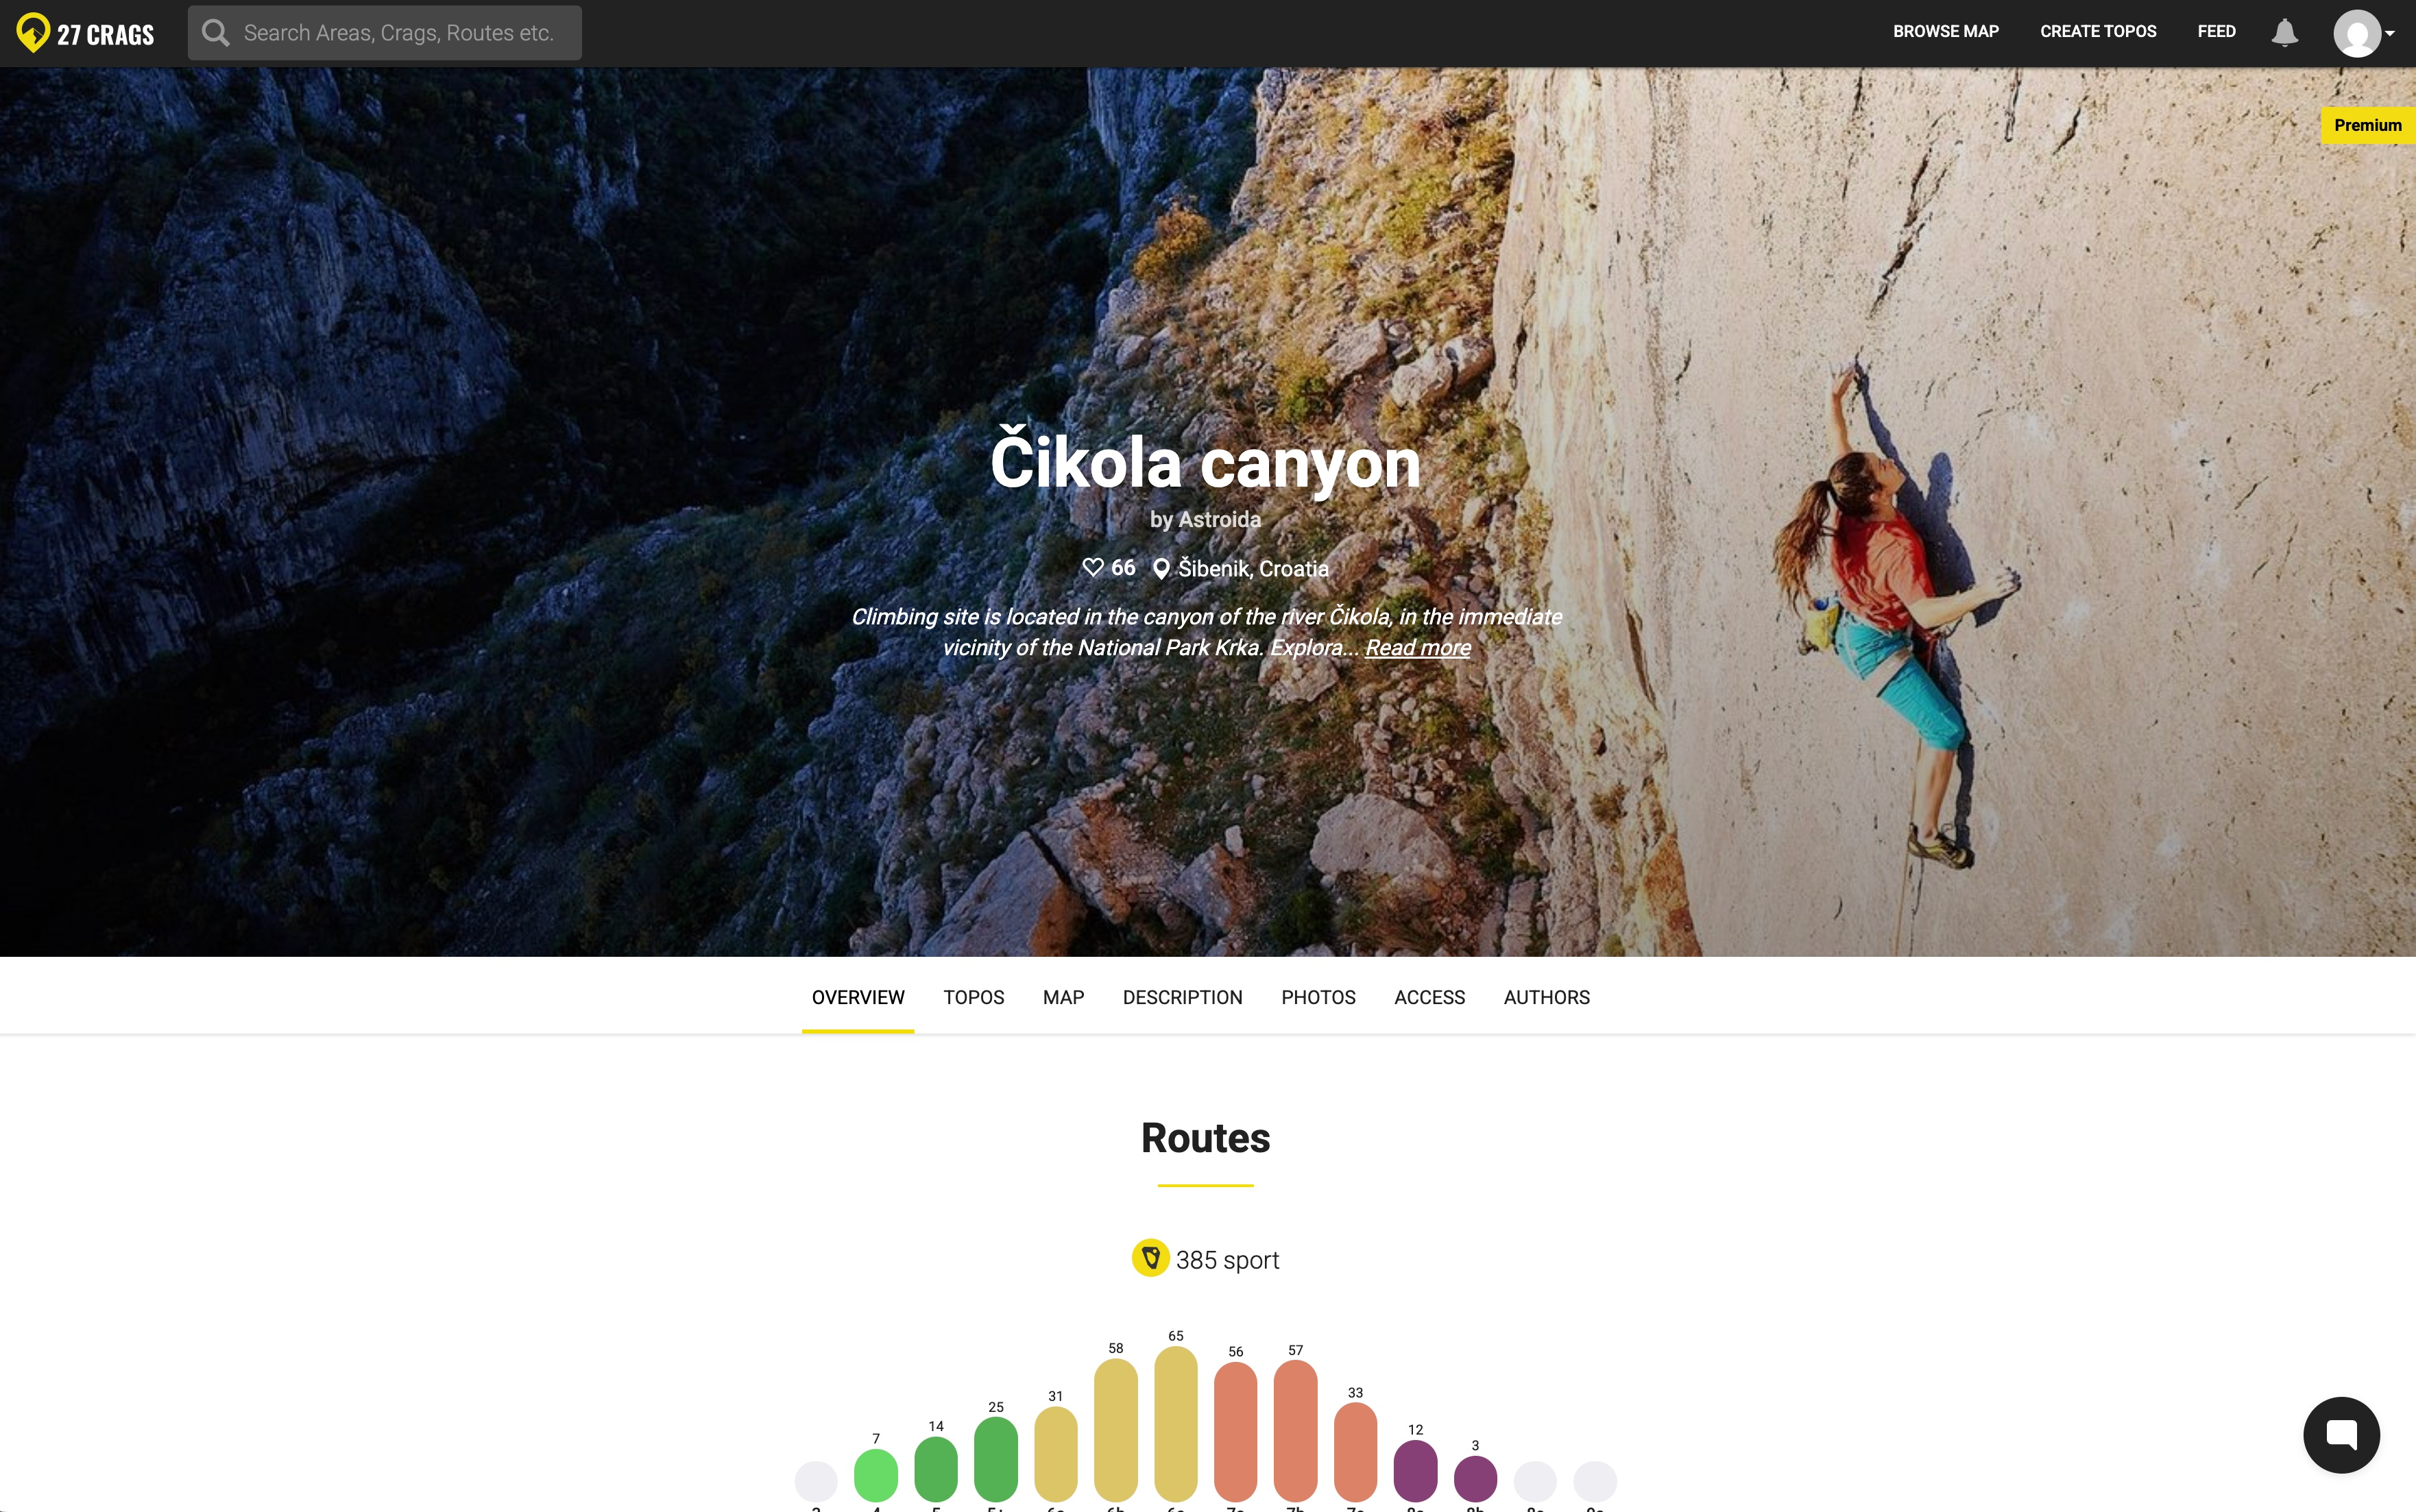
\includegraphics[width=0.75\textwidth]{images/uvod/27crags_cikola.jpeg}
    \caption{Prikaz penjačke lokacije Čikola na platformi \textit{27crags}}
\end{figure}
